\documentclass[10pt]{article}

\usepackage{parskip}
\usepackage[margin=1in]{geometry} 
\usepackage{tikz}
\usetikzlibrary{positioning}
\usepackage{amsmath,amsthm,amssymb, graphicx, multicol, array}
\usepackage{enumitem}
\usepackage{amssymb}
\usepackage{float}
\usepackage{href-ul}
 
\newcommand{\N}{\mathbb{N}}
\newcommand{\Z}{\mathbb{Z}}
 
\newenvironment{problem}[2][Problem]{\begin{trivlist}
\item[\hskip \labelsep {\bfseries #1}\hskip \labelsep {\bfseries #2.}]}{\end{trivlist}}

\begin{document}
 
\title{Instrumental Variables II}
\author{Jakob Sverre Alexandersen\\
GRA4158 Marketing and the Analysis of Experiments and Quasi-Experiments\\
Lecture 8}
\maketitle

\tableofcontents
\newpage

\section{Recap}

We use instrumental variables when:
\begin{itemize}
    \item Treatment allocation cannot be randomized 
    \item Time series are not available 
    \item Covariates are not available 
\end{itemize}

\subsection{Main idea}
\begin{itemize}
    \item \textbf{Basic idea:}
    \begin{itemize}
        \item $X_1 $ is never perfectly correlated with $ v $, this, there is variance in $X_1 $ that is uncorrelated with $v $
        \item Split the endogenous predictor variable $X_1 $ into two parts 
        \begin{itemize}
            \item One that is correlated with the error term (the one that causes $\mathbb{E}[v|X_1] \neq 0 $)
            \item One that is uncorrelated with the error term 
        \end{itemize}
        \item Use the uncorrelated part of $X_1 $ to estimate a consistent effect of $X_1 \text{ on } Y $
    \end{itemize}
    \item How to do the split?
    \begin{itemize}
        \item We can utilize an instrumental variable $Z $
        \item Must fulfill two important assumptions: 
        \begin{itemize}
            \item Intrument relevance: $\text{cov}(X_1, Z)\neq 0 $
            \item Intrument exogeneity: $\text{cov}(Z, v)  = 0 $
        \end{itemize}
    \end{itemize}
    \item In fact, the assumption implies that there are three different components in $X_1 $
    \item $X_1 = f(Z) + \rho v + \eta $
    \begin{itemize}
        \item An exogenous predictable part $f(Z)$
        \begin{itemize}
            \item The variation in $X $ that is explained by the instrument(s) $Z $, i.e., $\mathbb{E}[X_1|Z] $
        \end{itemize}
        \item An endogenous part $\rho v $
        \begin{itemize}
            \item This is the part of $X_1 $ that is related to the unobserved $v $ by the (regression/correlation) coefficient $\rho $ (if $\rho = 0 $ there is no endogeneity bias)
        \end{itemize}
        \item An idiosyncratic noise $\eta $
        \begin{itemize}
            \item It represents all the remaining variance in $X_1 $, i.e., all other reasons $X_1 $ cahnges that have nothing to do with your instrument $Z $, and nothing to do with the unobserved $v $ affecting $Y $
            \item The part os also exogenous but not predictable by $Z $
            \begin{itemize}
                \item It captures both variance related and unrelated to $Y $
            \end{itemize}
        \end{itemize}
    \end{itemize}
\end{itemize}
\newpage 
\subsection{How to estimate the model -- 2SLS -- idea}
\begin{itemize}
    \item First stage: 
    \begin{itemize}
        \item Regress $X_1 \text{ on } Z \to X_1 = \alpha + \gamma Z + \xi $ 
        \item Obtain predicted values $\mathbb{E}[X_1|Z] = \hat{X} = f(z) = \alpha + \gamma Z \quad $ requires that $\gamma \neq 0 $, i.e., $\text{cov}(X_1, Z) \neq 0 $
        \item The predicted values do not contain $\xi = \rho v + \eta $
        \item Remember: OLS implies that $\mathbb{E}[\xi|Z] = 0 $ and thus $\mathbb{E}[v|Z] = 0 \text{ and } \mathbb{E}[\eta|Z] = 0 $
    \end{itemize}
    \item Second stage: 
    \begin{itemize}
        \item Use these predicted $\hat{X}_1 $ to estimate the effect of $X \text{ on } Y $
        \item Estimate: $Y = \alpha + \beta_1\hat{X}_1 + \epsilon $
        \item Here: $\epsilon = \beta'\eta + v \text{ and } \mathbb{E}\left[\epsilon|\hat{X}_1\right] = 0 $
    \end{itemize}
    \item With: $\gamma \neq 0 $ (relevance; IV strength) and $\mathbb{E}[v|Z] = 0 $ (exclusion restriction; IV validity)
\end{itemize}
\subsection{The exogeneity condition / exclusion restriction}
\begin{figure}[H]
    \centering
    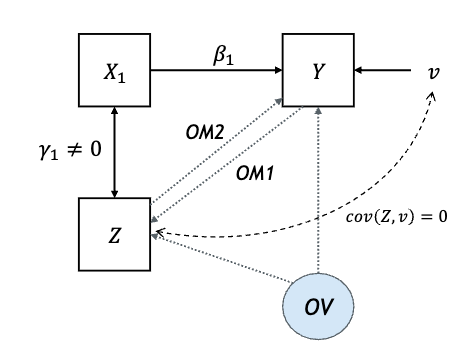
\includegraphics[width=0.4\textwidth]{2026-03-06-11-03-36.png}
\end{figure}
\begin{itemize}
    \item The exogeneity condition has three implications
    \begin{itemize}
        \item No OM1: No omitted meachinisms enabling the IV to affect the dependent variable directly or indirectly that is not through $X_1 $
        \item No OM1: No omitted meachinisms enabling the dependent variable to affect the IV (i.e., any form of reverse-causality)
        \item No OVs: No omitted variables affecting both the IV and the dependent vairable 
    \end{itemize}
    \item These assumptions are ususally not testable, but require careful judgement by the researcher
\end{itemize}

\newpage 
\section{Several endogenous, exogenous and instrumental variables}
\begin{itemize}
    \item The focal regression equation: $Y = \alpha + \beta_1X_1 + \beta_2X_2 + \beta_3W_3 + \beta_4W_4 + \epsilon $
    \begin{itemize}
        \item $X_1 \text{ and } X_2 $ are both endogenous (i.e., $\mathbb{E}[\epsilon|X_1, X_2]\neq 0 $); $W_1 \text{ and } W_2 $ are both exogenous (i.e., $\mathbb{E}[\epsilon|W_1, W_2] = 0 $)
        \item We have three instruments $Z_1, Z_2, Z_3 $ with $\text{cov}(\epsilon, Z) = 0 \text{ and cov}(\epsilon, X)\neq 0 $
    \end{itemize}
    \item First stage: Regress all instruments $Z $ and all exogenous $W $ on all $X $
    \begin{itemize}
        \item Estimate $X_1 =\gamma_0 + \gamma_1W_1 + \gamma_2W_2 + \gamma_3Z_1 + \gamma_4Z_2 + \gamma_4Z_3 + \psi$
        \item Estimate $X_2 =\omega_0 + \omega_1W_1 + \omega_2W_2 + \omega_3Z_1 + \omega_4Z_2 + \omega_4Z_3 + \psi$
        \item Obtain predicted values $\hat{X}_1 \text{ and }\hat{X}_2 $
    \end{itemize}
    \item Second stage: Replace $X_1\text{ and }X_2 $ with predicted values $\hat{X}_1 \text{ and }\hat{X}_2 $
    \begin{itemize}
        \item Estimate $Y = \alpha + \beta_1\hat{X}_1 + \beta_2\hat{X}_2 + \beta_3W_1 + \beta_4W_2 + \epsilon $
        \item $\beta_1\text{ and }\beta_2 $ are consistent if $Z_1, Z_2, Z_3 $ fulfill the instrumental variable assumptions 
    \end{itemize}
\end{itemize}
\textbf{Some key aspects}
\begin{itemize}
    \item We always need at least as many instruments $Z $ as endogenous variables $X $
    \begin{itemize}
        \item i.e., in the previous example we would need at least two (but we have three)
    \end{itemize}
    \item We always use \textbf{all instruments} for all endogenous variables in the first stage regressions
    \begin{itemize}
        \item If an instrument is not relevant, regression will sort it out with a zero coefficient
        \item At least one instrument needs to be relevant for each endogenous variable 
        \item With multiple endogenous variables we have different relevance tests
    \end{itemize}
    \item We always include all (exogenous) covariates in the first stage regressions 
\end{itemize}
\newpage 
\section{Testing the strength / relevance of instruments}
\begin{figure}[H]
    \centering
    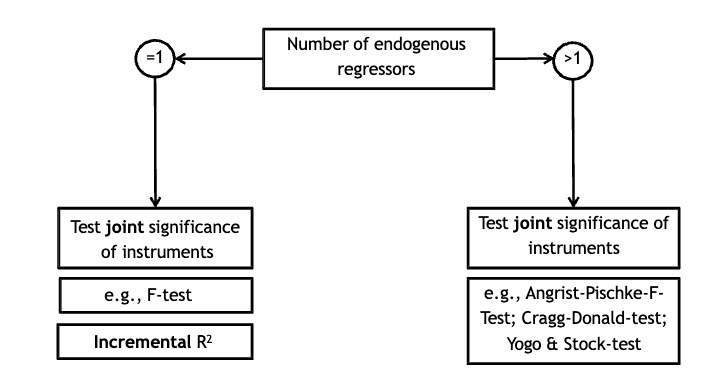
\includegraphics[width=0.7\textwidth]{2026-03-06-12-37-45.png}
\end{figure}
\subsection{Testing the exogeneity condition -- Sargan test}
\begin{itemize}
    \item As stated before, we usually cannot test directly whether the exogeneity assumption holds 
    \begin{itemize}
        \item We need to use economic theory and expert knowledge to justify the validity of instruments 
    \end{itemize}
    \item In the special case where more IVs than endogenous variables are available (i.e., the model is overidentified), overidentification tests can shed some light on the adequacy of instruments: the Sargan test or the Hansen J-test 
    \begin{itemize}
        \item However, many problems remain 
        \begin{itemize}
            \item When \underline{all} instruments are invalid, the test will be biased, and inference may be wrong 
            \item They test the joint hypothesis of instrument validity and correct functional form 
            \begin{itemize}
                \item If the test fails, we don't know why (which instrument is invalid or if functional form is invalid)
            \end{itemize}
            \item The power of the tests are rather low (high chance of not rejecting $H_0 $ when IVs are invalid)
        \end{itemize}
    \end{itemize}
\end{itemize}
\newpage 
\section{Variations from the basic linear model}
\begin{itemize}
    \item Interactions and quadratic terms of the endogenous regressor $X $ need special treatment in the first stage and second stage making the procedure more complicated 
    \begin{itemize}
        \item Often, researchers rely on the \textit{control function approach} in such cases
    \end{itemize}
    \item Binary endogenous $X $ (e.g., treatment vs. control; buy vs. not buy) and continuous instruments 
    \begin{itemize}
        \item You can do the standard approach using OLS (linear probability model; however, predicted $X $ might be out of the range 0-1)
        \begin{itemize}
            \item Some strong proponents and some strong critics of this approach 
        \end{itemize}
        \item Alternative could be to first estimate a probit model and use predicted probabilities as instruments in the first stage regression
        \begin{itemize}
            \item This approach can be more efficient than direct 2SLS 
        \end{itemize}
    \end{itemize}
\end{itemize}
\section{Control function approach -- an alternative to 2SLS}
\begin{itemize}
    \item First stage is the same as 2SLS 
    \begin{itemize}
        \item However, we do not use the predicted values $\hat{X} $, but the regression residual $\hat{\xi} $ from the first stage as additional regressor (control function)
        \item Estimate: $Y = \alpha + \beta X + \rho\hat{\xi} + \epsilon $ 
    \end{itemize}
    \item Idea
    \begin{itemize}
        \item Instead of using the exogenous (uncorrelated) variance of $X $ to estimate the effect, we include the endogenous variance (the correlated part $\rho v $) as additional control variable
        \item Our model now controls for the unobserved variation that makes $X $ endogenous
        \item The effect of $X $ should then represent only the part that is not correlated with the error term 
    \end{itemize}
\end{itemize}
\subsection{Important aspect}
\begin{itemize}
    \item The control function approach makes the same assumptions on instrments $Z $ as 2SLS 
    \begin{itemize}
        \item relevance and exogeneity condition!
    \end{itemize}
    \item If the coefficient of the residual is significant, this indicates the pre poopoo
\end{itemize}
\end{document}